\documentclass{beamer}
%\documentclass[handout,t]{beamer}

\usepackage{pgfpages}
\pgfpagesuselayout{4 on 1}[letterpaper,landscape,border shrink=5mm]

\usepackage{amsmath,amssymb,enumerate,epsfig,bbm,calc,color,ifthen,capt-of}

\usetheme{metropolis}

\title{Underwater Real-Time Object Recognition and Tracking for
Autonomous Underwater Vehicle}
\author{Tan Soon Jin}
\institute[National University of Singapore]{Department of Computer Science}

\date{\today}

\beamerdefaultoverlayspecification{<+->}
\begin{document}
% ----------------- Title -----------------------------------------------------
\frame{\titlepage}
% -----------------------------------------------------------------------------

% Section 1: Motivation -------------------------------------------------------
\section{Motivation}

\subsection{Underwater Real-Time Object Tracking}
\begin{frame}{Underwater Real-Time Object Tracking}
    \begin{figure}[ht]
        \centering
        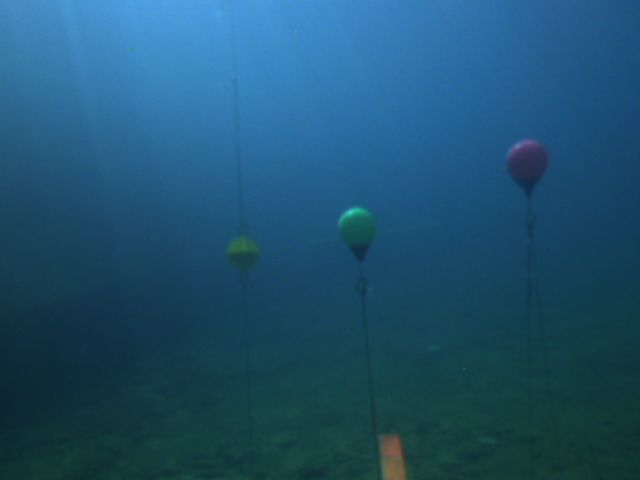
\includegraphics[width=0.3\textwidth, height=0.3\textwidth]{figs/robosub16_buoy_bluish.png}
    \end{figure}
    Develop a \textit{flexible} and \textit{robust} real-time object tracking framework that will be deployed in the \textit competition.
\end{frame}

\subsection{Problems}
\begin{frame}{Problems}
    \begin{itemize}
        \item Human in the loop
            \begin{enumerate}
                \item Manual tuning of algorithms parameters i.e color threshold
                \item Choosing algorithms that for a particular water condition
                \item Tuning camera parameters to ensure decent image input
            \end{enumerate}
        \item Typically, expensive sensors i.e sonar and stereo camera required to achieve robust object tracking.
    \end{itemize}
\end{frame}

\subsection{Our approach}
\begin{frame}{Our approach}
    \begin{figure}[ht]
        \centering
        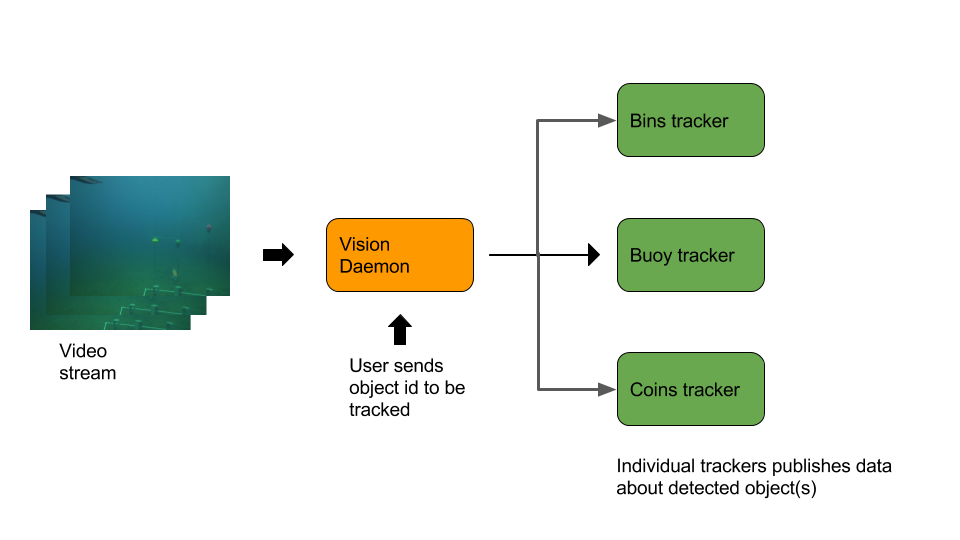
\includegraphics[width=0.5\textwidth]{figs/overall_vision_architecture.png}
    \end{figure}
    \begin{enumerate}
        \item A highly modular and robust object tracking module managed by a vision daemon.
        \item Emphasis on preprocessing in combination with simple and efficient computer vision techniques.
        \item Automatic parameter tuning and model selection.
    \end{enumerate}
\end{frame}

% -----------------------------------------------------------------------------

% Section 2: Key Idea ---------------------------------------------------------

\section{Key Idea}

\subsection{Vision arbiter}
\begin{frame}{Vision arbiter}
    \begin{figure}[ht]
        \centering
        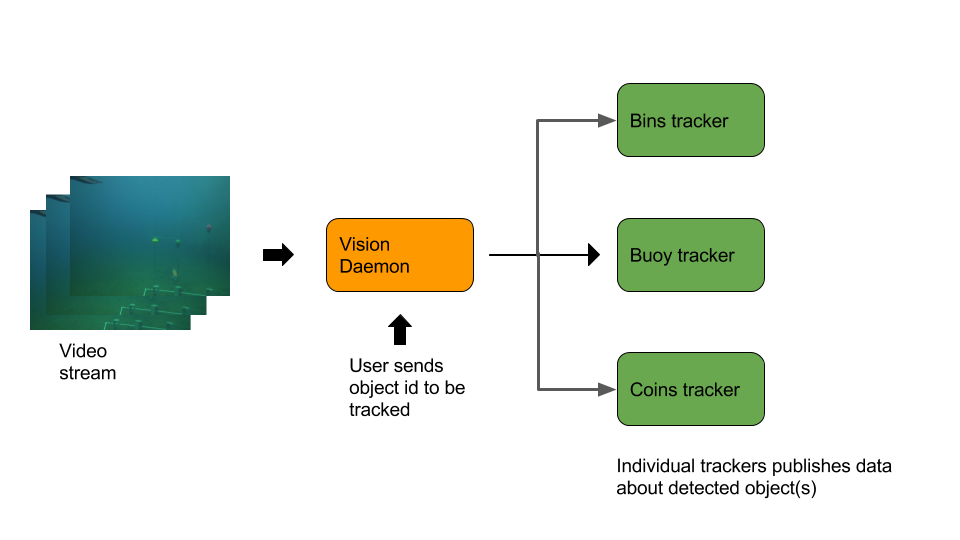
\includegraphics[width=0.5\textwidth]{figs/overall_vision_architecture.png}
    \end{figure}
    Running a vision service that allow for specifying object specific configurations for multiple-object tracking. Ease of use.
\end{frame}

\subsection{Taking human out of the loop}
\begin{frame}{Taking human out of the loop (Work in progress)}
    \begin{figure}[ht]
        \centering
        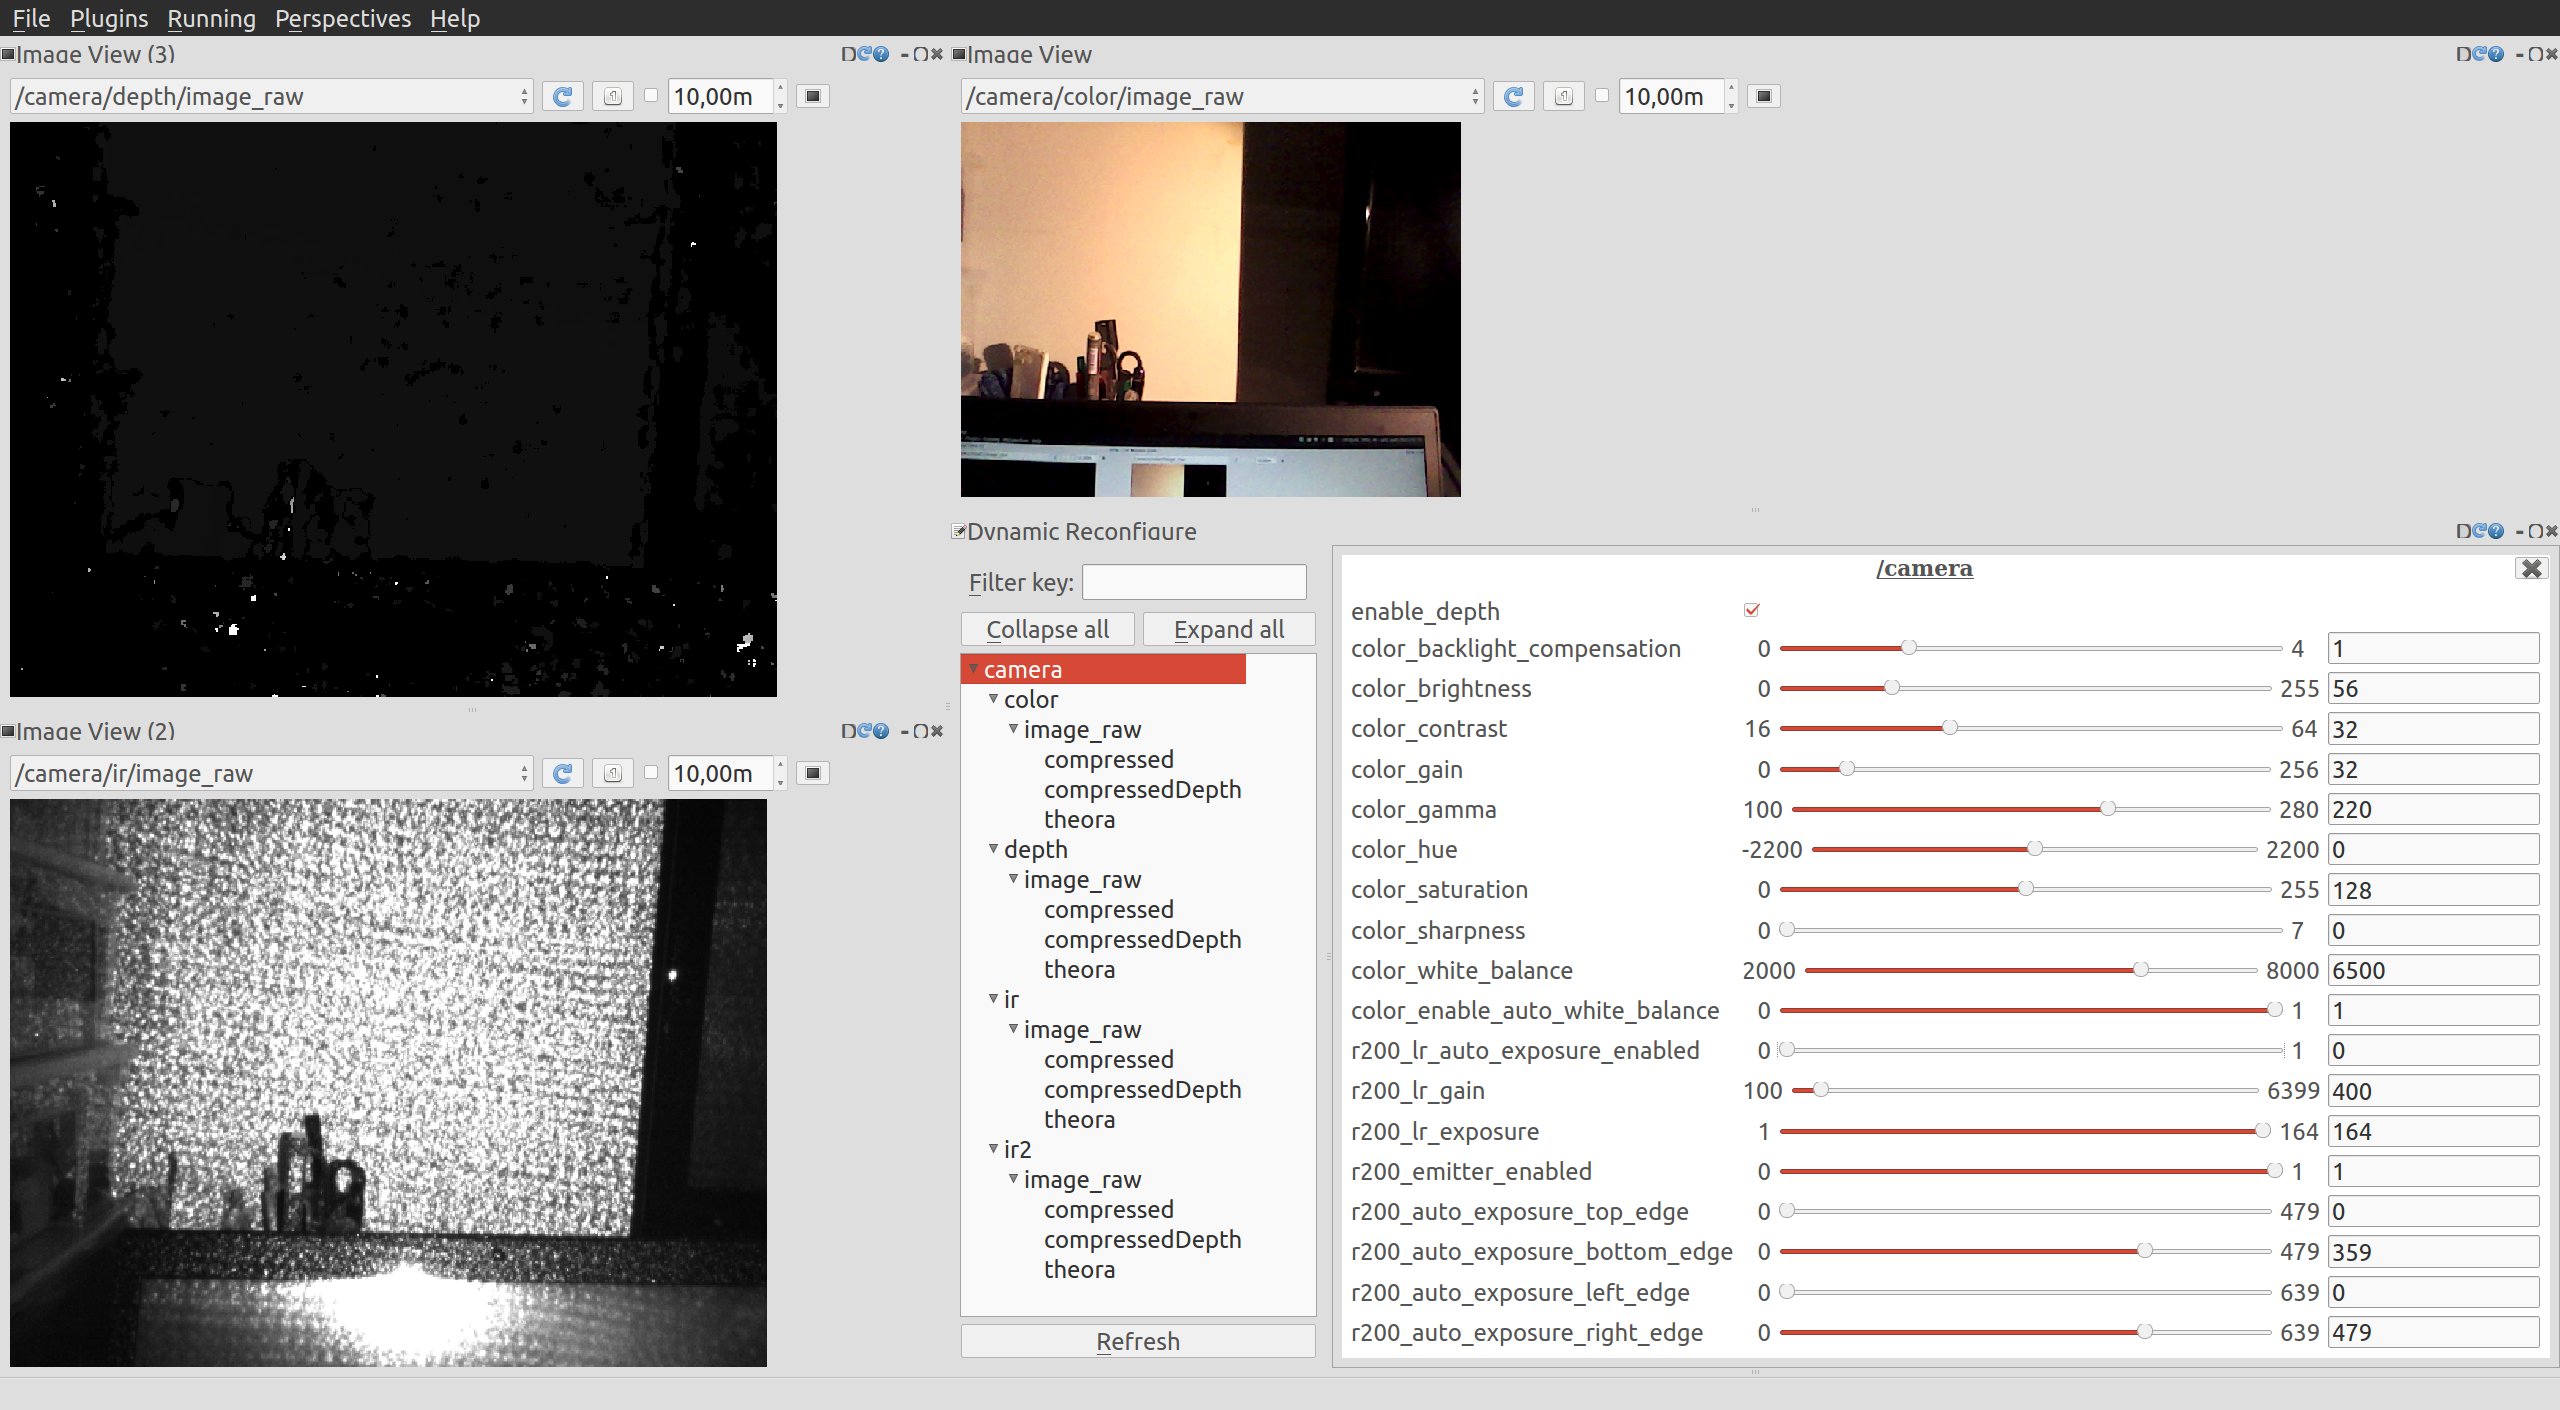
\includegraphics[width=0.4\textwidth, height=0.4\textheight]{figs/dynamic_reconf.png}
    \end{figure}
    \begin{enumerate}
        \item Dynamic camera parameters tuning based on image statistics i.e mean intensity of image
    \end{enumerate}
\end{frame}

% ----------------------------------------------------------------------------

% Section 3: Background ------------------------------------------------------

\section{Background}

\subsection{About Robosub}
\begin{frame}{About Robosub}
    \begin{figure}[ht]
        \centering
        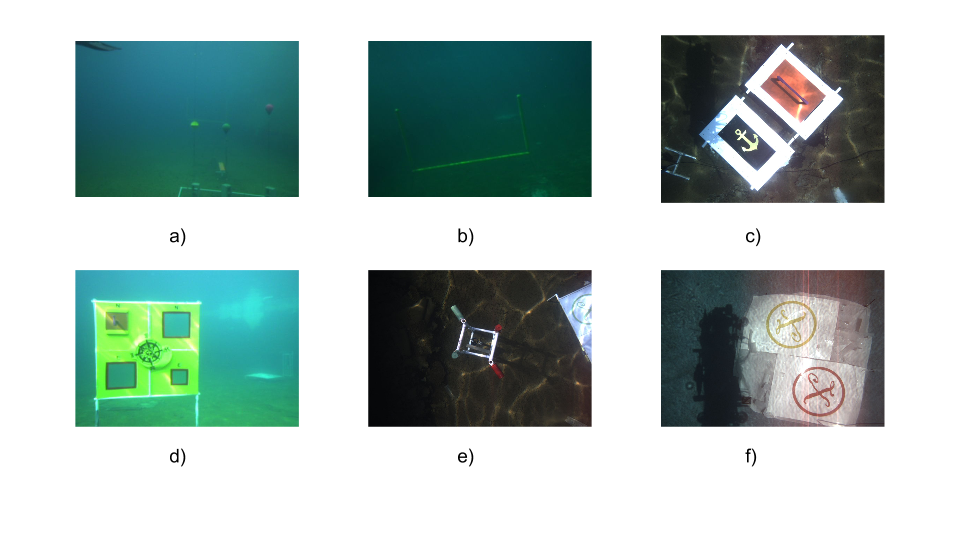
\includegraphics[width=0.6\textwidth, height=0.5\textheight]{figs/robosub_vision_tasks.png}
    \end{figure}
    AUV (Autonomous Underwater Vehicle) built by university students are challenged to complete a series of underwater tasks that mimic real-world applications.
\end{frame}

\subsection{Underwater computer vision}
\begin{frame}{Underwater computer vision}
    \begin{figure}[ht]
        \centering
        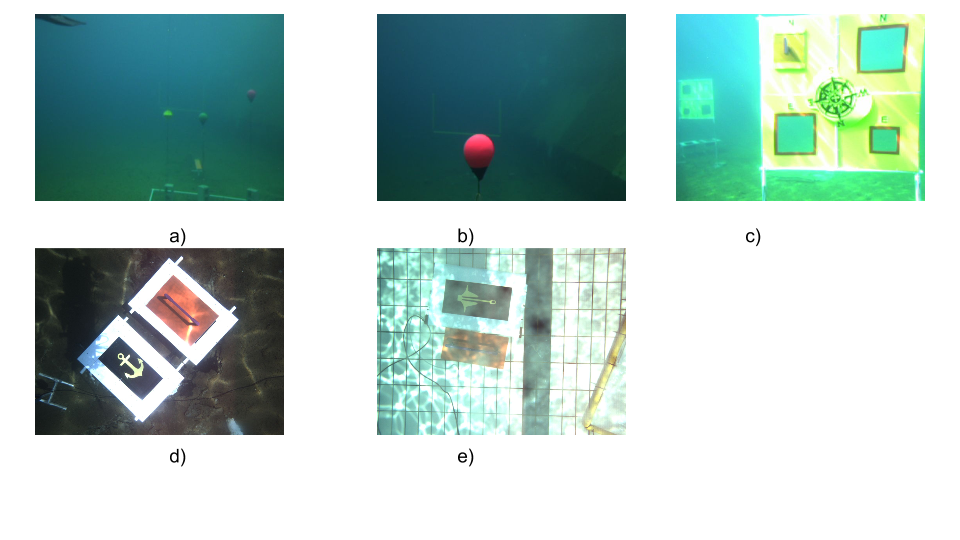
\includegraphics[width=0.6\textwidth, height=0.5\textheight]{figs/task_challenges.png}
    \end{figure}
    \begin{itemize}
        \item Color degradation due to scattering of light. Red appears darker and bluish-green hue
        \item Low contrast because of haze formation
    \end{itemize}
\end{frame}

\begin{frame}{Underwater computer vision (cont'd)}
    \begin{description}
        \item[Low contrast] Object loses such as edges and texture
        \item[Partial occlusion] Object temporarily occluded by small object
        \item[Non-uniform illumination] Certain part of object is overexposed
    \end{description}
\end{frame}

\subsection{Related Work}
\begin{frame}{Related Work}
    \begin{figure}
        \centering
        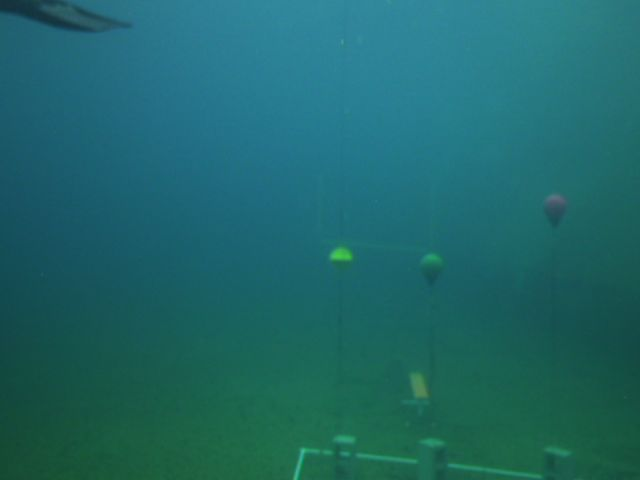
\includegraphics[width=0.3\textwidth, height=0.3\textheight]{figs/robosub16_buoy_hazy.png}\hspace{5em}
        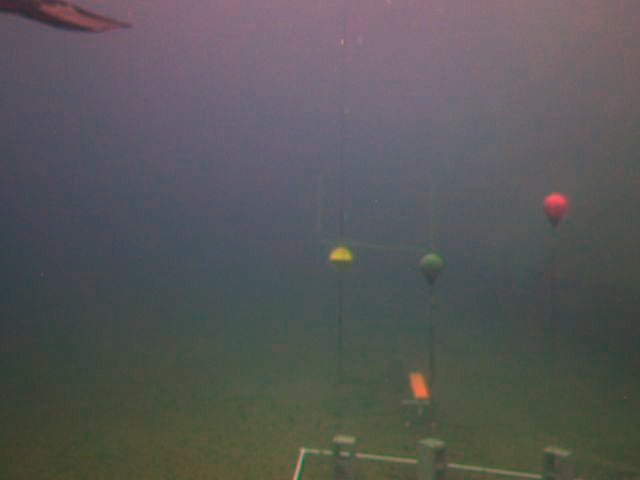
\includegraphics[width=0.3\textwidth, height=0.3\textheight]{figs/robosub16_buoy_hazy_shadegrey.png}
    \end{figure}
    \begin{itemize}
        \item How the human perception system ensures color of objects remain relatively constant under different illuminations.
        \item Shade of grey, Gray World, White-Patch
    \end{itemize}
\end{frame}

\begin{frame}{Related Work}
    \begin{enumerate}
        \item \textbf{Gamma correction:} Non-linear transformation of raw image to match human perception.
        \item \textbf{Homomorphic filter:} Remove sunlight flicker assuming high frequency component corresponds to true illumination of the object.
    \end{enumerate}
\end{frame}

\begin{frame}{Related Work}
        \begin{figure}
            \centering
            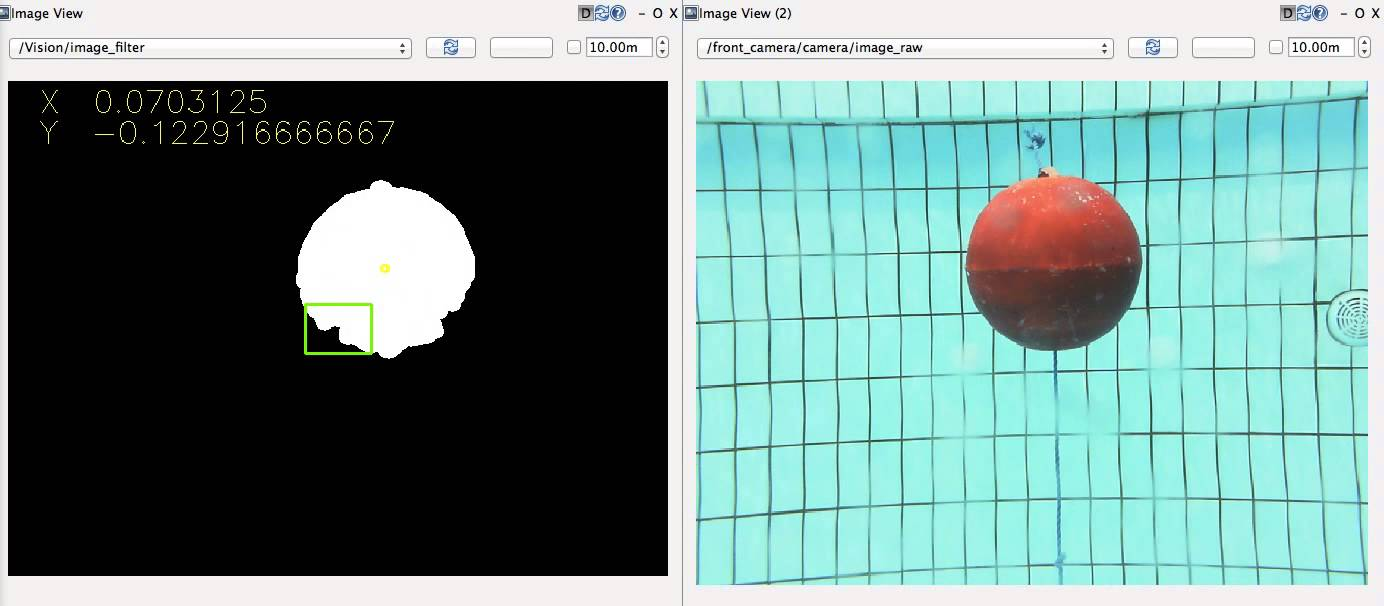
\includegraphics[width=0.5\textwidth]{figs/blob_detection.jpg}
        \end{figure}
        \begin{enumerate}
            \item \textbf{Feature Extraction:} Colour, Edge, Shape
            \item \textbf{Feature Matching:} Similarity measure, Geometrical Constraints
        \end{enumerate}
\end{frame}

\begin{frame}{Related Work}
        \begin{figure}
            \centering
            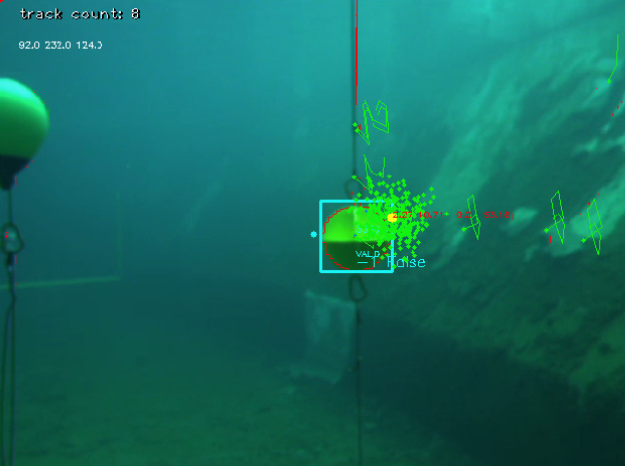
\includegraphics[width=0.3\textwidth]{figs/pf_buoy_0.png}\hspace{5em}
            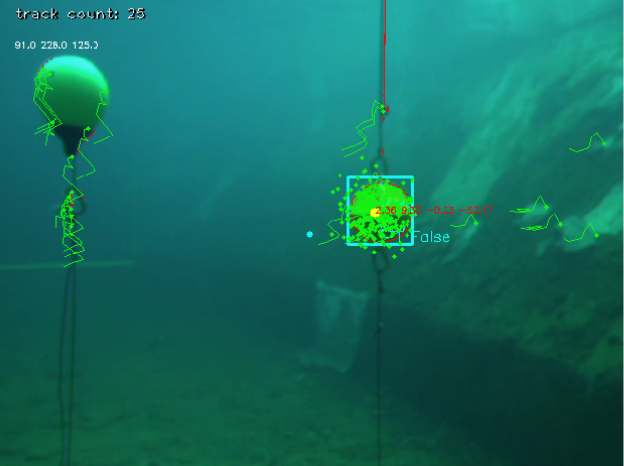
\includegraphics[width=0.3\textwidth]{figs/pf_buoy_1.png}
        \end{figure}
        \begin{enumerate}
            \item Represents a distribution as a set of weighted particles.
            \item Update \to Predict \to Resample
        \end{enumerate}
\end{frame}

% ----------------------------------------------------------------------------

% Section 4: Object Tracking -------------------------------------------------

\section{Object Tracking Pipeline}

\subsection{Overview}
\begin{frame}{Object Tracking Pipeline}
    \begin{figure}[ht]
        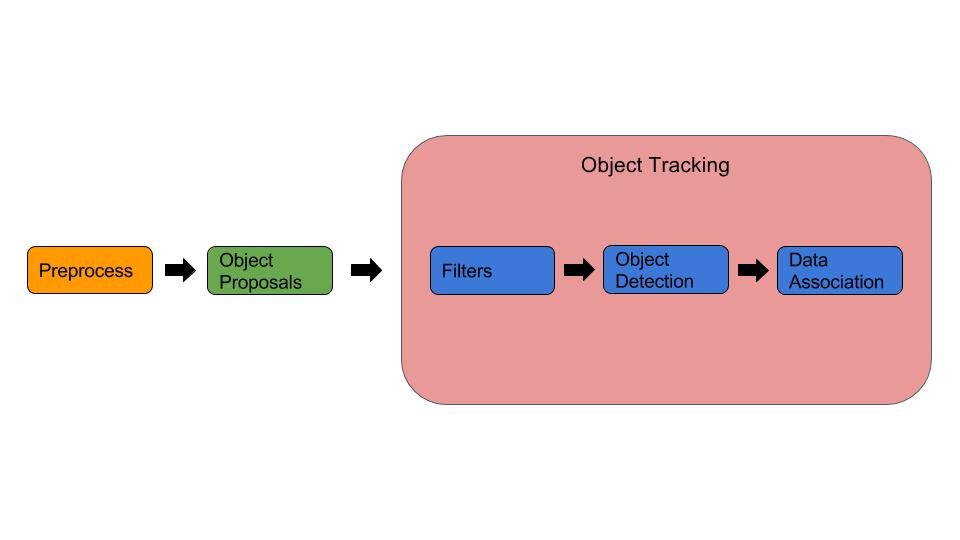
\includegraphics[width=0.7\textwidth]{figs/tracker_pipeline.jpg}
    \end{figure}
\end{frame}

\subsection{Preprocessing}
\begin{frame}{Preprocessing}
    \begin{figure}[ht]
        \centering
        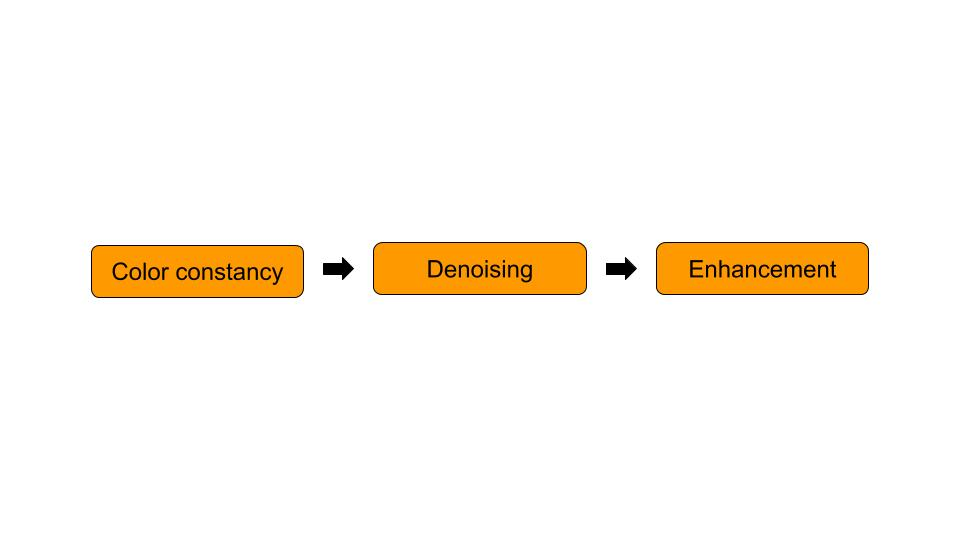
\includegraphics[width=0.7\textwidth, height=0.5\textheight]{figs/preprocess_pipeline.jpg}
    \end{figure}
    \textit{Note:} Some steps are performed on demand and may be skipped depending on test environment.
\end{frame}

\begin{frame}{Preprocessing}
    \begin{figure}[ht]
        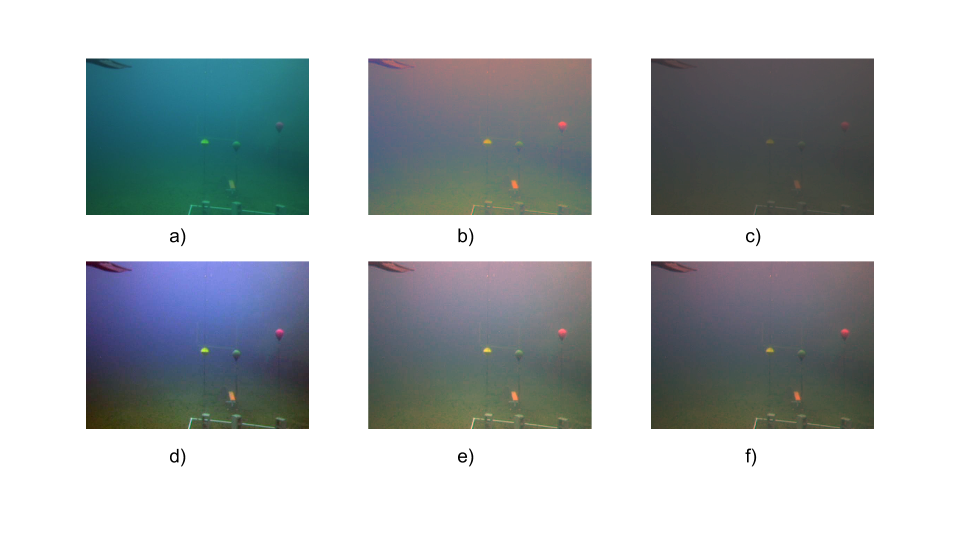
\includegraphics[width=0.7\textwidth, height=0.5\textheight]{figs/color_constancy.png}
    \end{figure}
    \begin{itemize}
        \item Uses low-level statistics methods. Fast \& Simple.
        \item How important is the accuracy of recovered image for further processing ?
    \end{itemize}
\end{frame}

\begin{frame}{Preprocessing}
    \begin{figure}[ht]
        \centering
        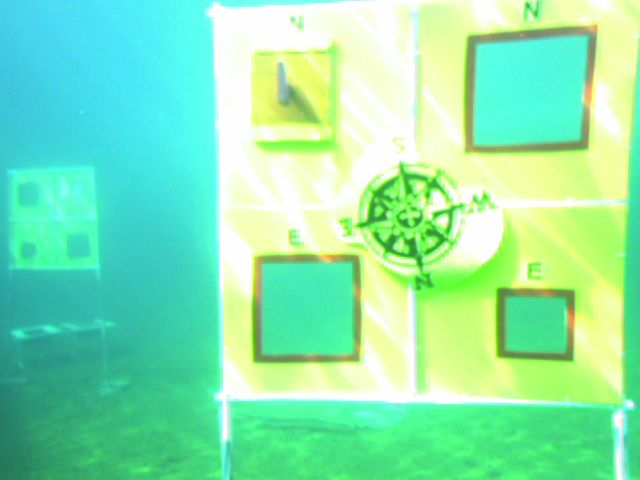
\includegraphics[width=0.3\textwidth, height=0.3\textheight]{figs/robosub16_torpedo_orange_yellow_superbright.png}\hspace{5em}
        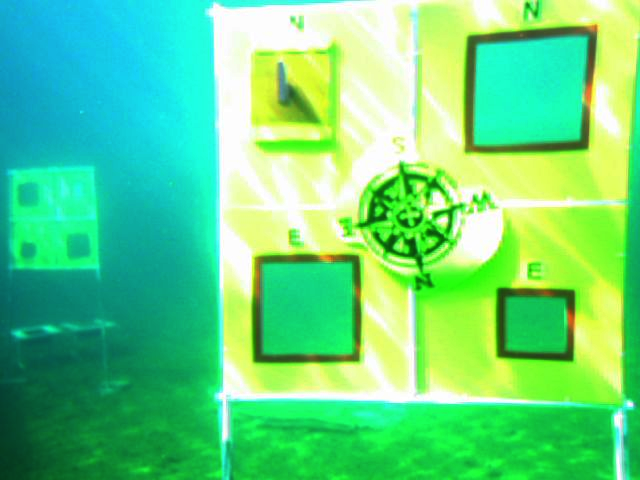
\includegraphics[width=0.3\textwidth, height=0.3\textheight]{figs/robosub16_torpedo_orange_yellow_superbright_gamma_correct.png}
    \end{figure}
    Correct sudden change in illumination i.e sun is directly over the obstacle.
\end{frame}

\begin{frame}{Preprocessing}
    \begin{figure}[ht]
        \centering
        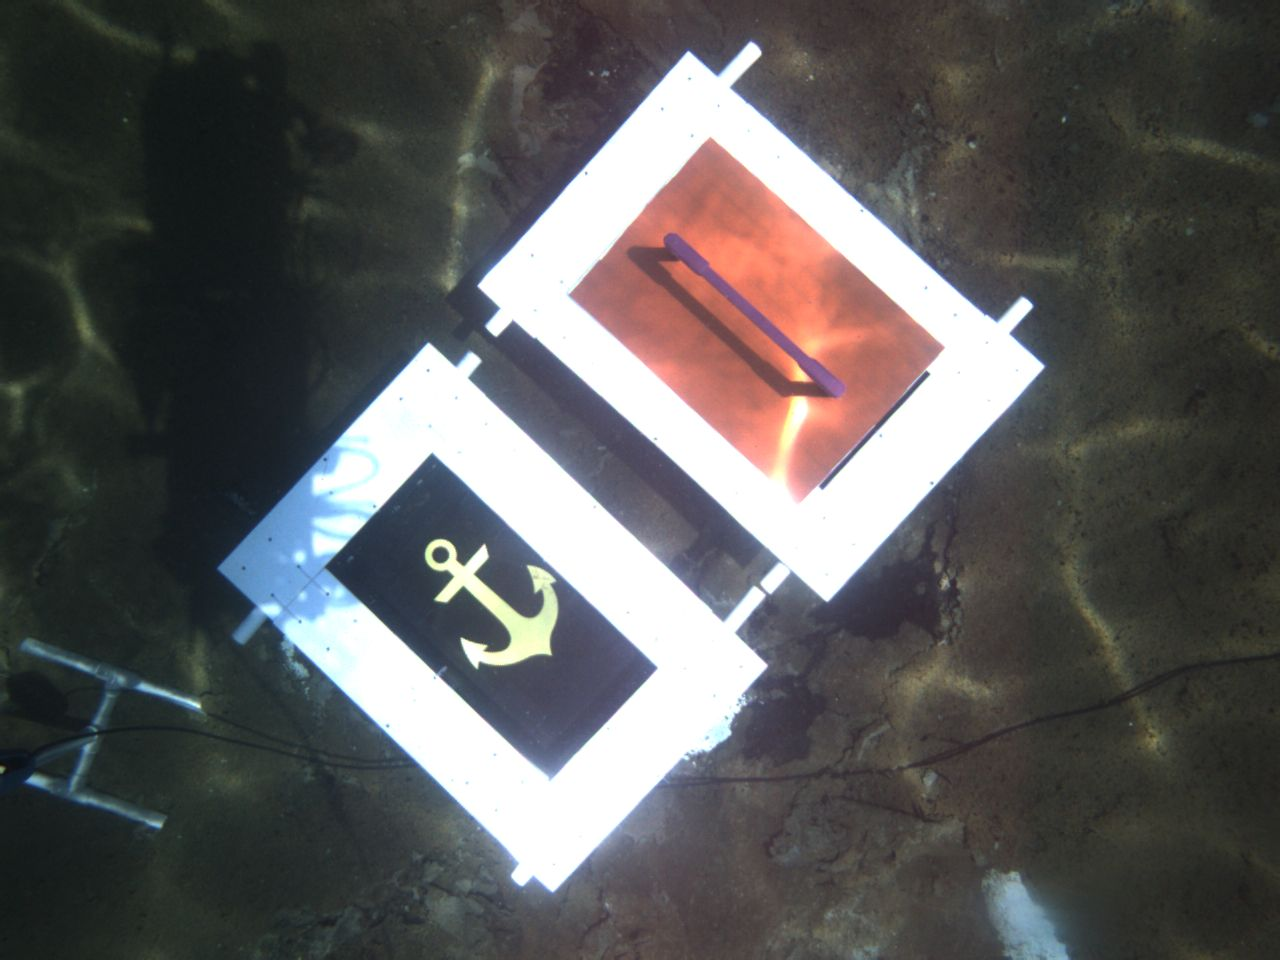
\includegraphics[width=0.3\textwidth, height=0.3\textheight]{figs/robosub16_bin_flicker_shadow.png}\hspace{5em}
        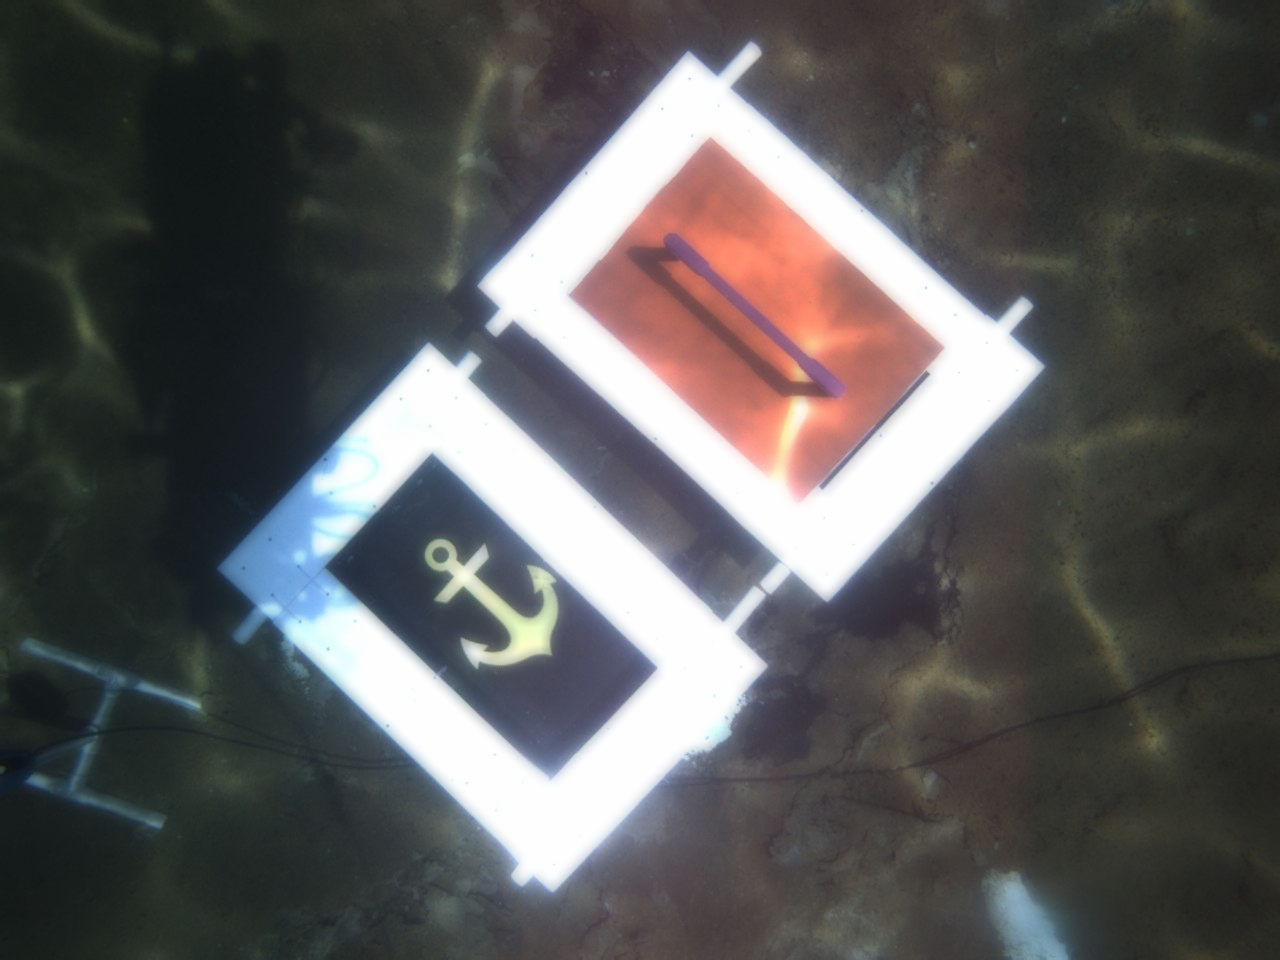
\includegraphics[width=0.3\textwidth, height=0.3\textheight]{figs/robosub16_bin_flicker_shadow_homomorphic_filter.png}
    \end{figure}
    Reduces intensity of sunlight flickering to recover details of obstacle.
\end{frame}

\begin{frame}{Preprocessing}
    \begin{figure}[ht]
        \centering
        
\includegraphics[width=0.3\textwidth, height=0.3\textheight]{figs/pole_blur.png}\hspace{5em}
        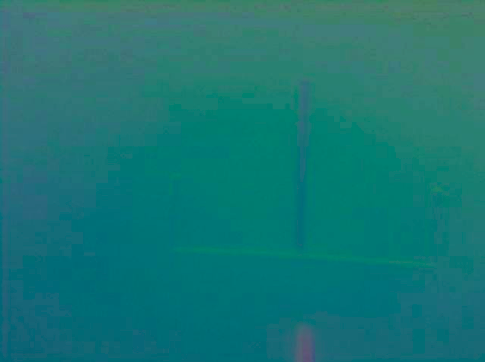
\includegraphics[width=0.3\textwidth, height=0.3\textheight]{figs/pole_enhance.png}
    \end{figure}
    Recover details such as edges and color that are lost because of backscattering of light.
\end{frame}

\subsection{Generating object candidates}
\begin{frame}{Generating object candidates}
        \begin{figure}[ht]
        \centering
            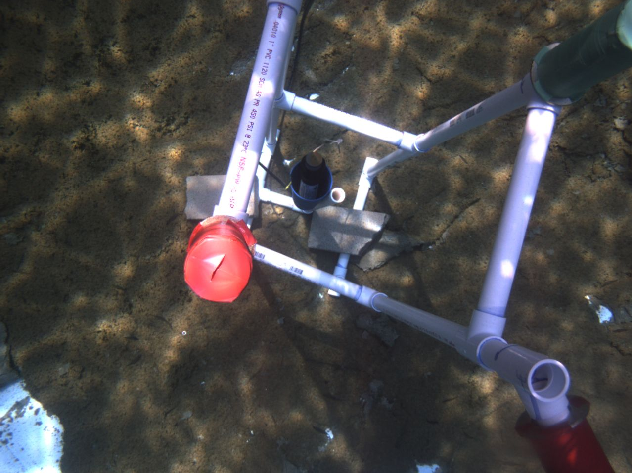
\includegraphics[width=0.3\textwidth, height=0.3\textheight]{figs/redcoin.png}\hspace{5em}
            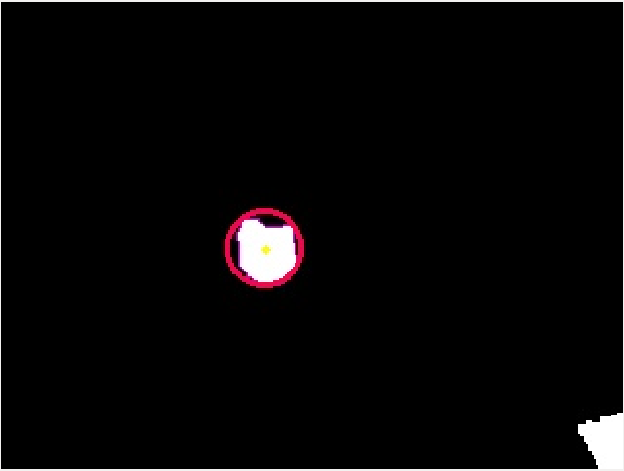
\includegraphics[width=0.3\textwidth, height=0.3\textheight]{figs/redcoin_blob.png}
    \end{figure}
    \begin{itemize}
        \item Color thresholding. Multiple-color space.
        \item Edge detection.
    \end{itemize}
\end{frame}

\begin{frame}{Generating object candidates}
    \begin{figure}[ht]
        \centering
        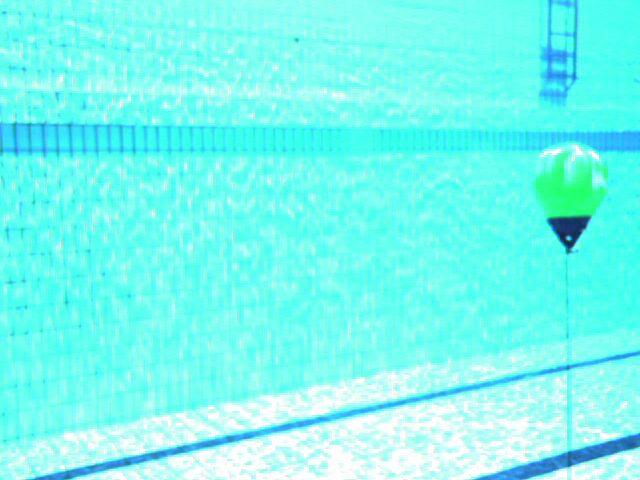
\includegraphics[width=0.3\textwidth, height=0.3\textheight]{figs/qt16_buoy_bright_green.png}\hspace{5em}
        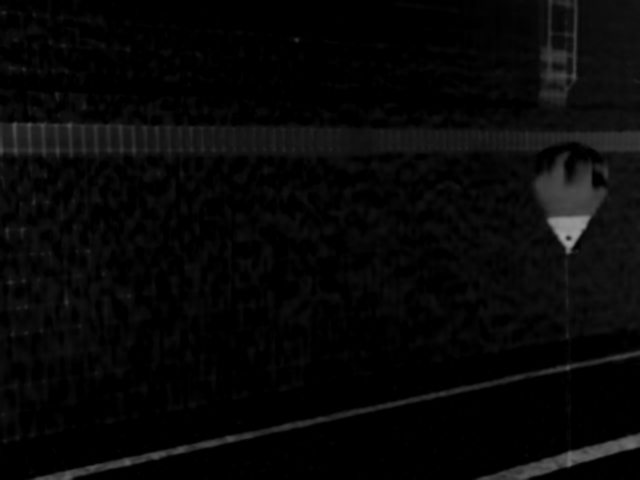
\includegraphics[width=0.3\textwidth, height=0.3\textheight]{figs/qt16_buoy_bright_green_saliency.png}
    \end{figure}
    Detects visual cues that distinct with respect to its surrounding.
\end{frame}

\subsection{Filtering}
\begin{frame}{Filtering}
    \begin{enumerate}
        \item Geometrical constraints i.e rectangle, circle
        \item Aspect-ratio
        \item Size
        \item Methodology:
            \begin{itemize}
                \item Sequential
                \item Parallel
            \end{itemize}
    \end{enumerate}
\end{frame}

\subsection{Data association}
\begin{frame}{Data association: Nearest Neighbor Approach}
    \begin{figure}[ht]
        \centering
        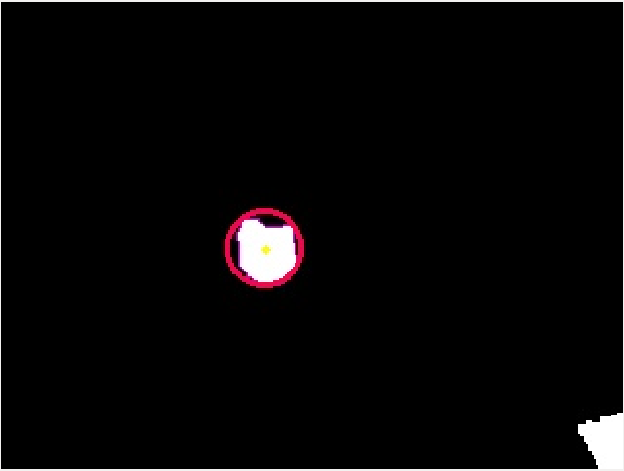
\includegraphics[width=0.3\textwidth, height=0.3\textheight]{figs/redcoin_blob.png}\hspace{5em}
        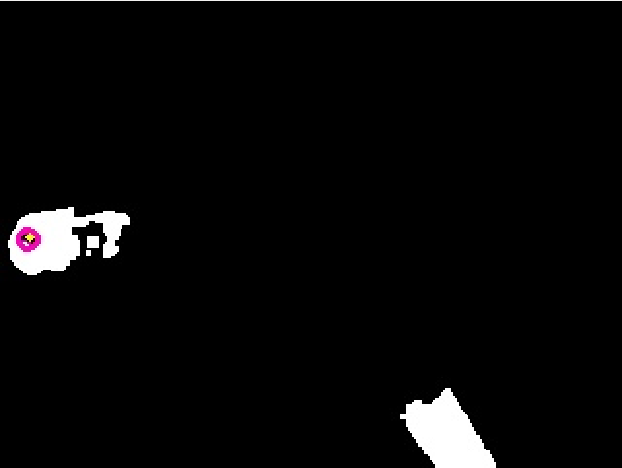
\includegraphics[width=0.3\textwidth, height=0.3\textheight]{figs/redcoin_next.png}
    \end{figure}
    Chooses detected object that is closest to previously tracked object.
\end{frame}

% ----------------------------------------------------------------------------

% Section 5: Vision framework ------------------------------------------------

\section{Vision Framework}

\subsection{Overview}
\begin{frame}{Vision Framework}
    \begin{figure}[ht]
        \centering
        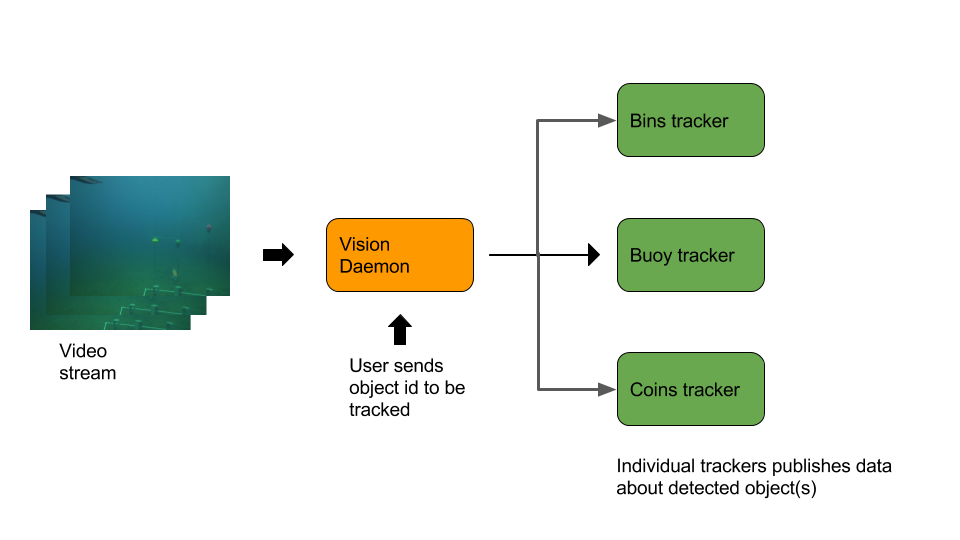
\includegraphics[width=0.4\textwidth]{figs/overall_vision_architecture.png}\hspace{5em}
        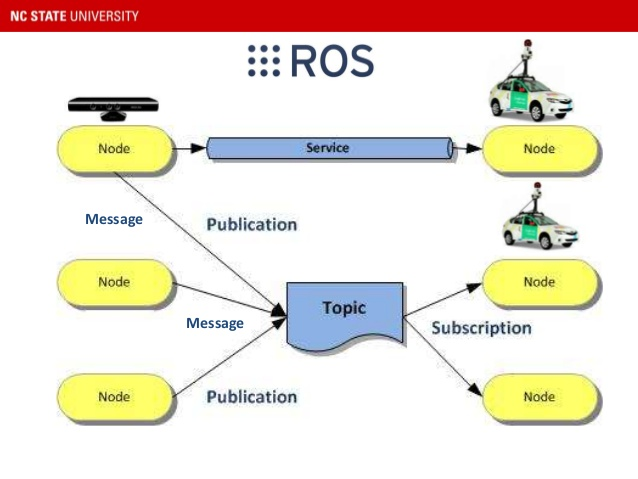
\includegraphics[width=0.4\textwidth]{figs/ros_details.jpg}
        \caption{Credits to NC State university for ROS picture}
    \end{figure}    
\end{frame}

% ----------------------------------------------------------------------------

% Section 6: Automatic hyperparameter tuning ---------------------------------

\section{Taking human out of the loop}

\subsection{Automatic hyperparameter tuning}
\begin{frame}{Automatic hyperparameter tuning}
    \begin{figure}[ht]
        \centering
        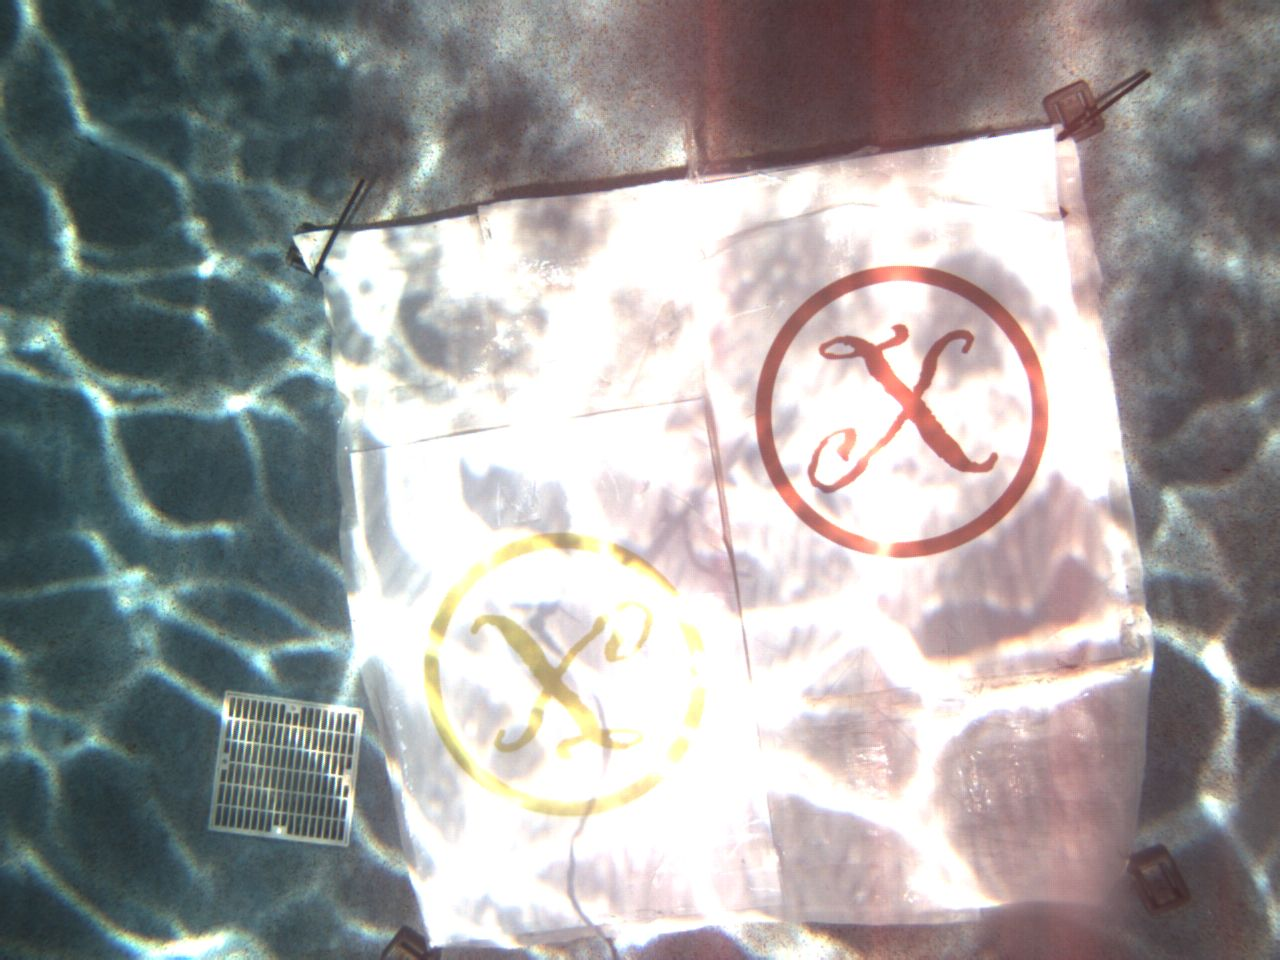
\includegraphics[width=0.4\textwidth]{figs/sundale_table_flicker.png}\hspace{5em}
        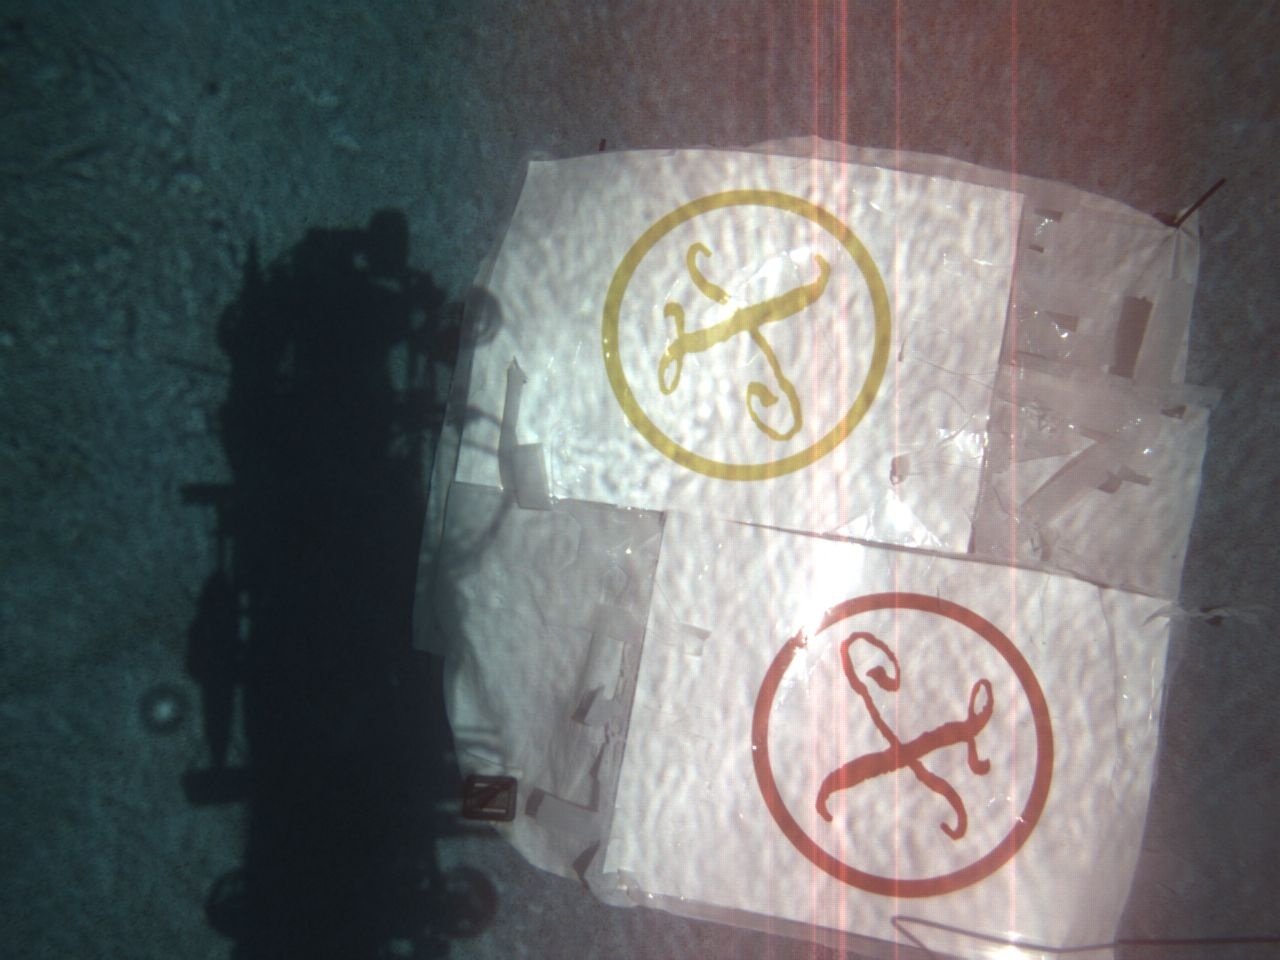
\includegraphics[width=0.4\textwidth]{figs/sundale_table_shadow.png}
    \end{figure}   
    Automatically adjusts parameters of camera to adapt to change in surrounding environment.
\end{frame}

% ----------------------------------------------------------------------------

% Section 7: Experiment Evaluations ------------------------------------------
\section{Experiment evaluations}

\subsection{Evaluating the baseline}
\begin{frame}{Evaluating the baseline}
    \begin{enumerate}
        \item Testing the baseline methods on \textit{Robosub 2016} dataset, baseline achieves accuracy of approximately 50\% of successfully tracked frames.
        \item Evaluation is performed through human observation on
        \item Propose more accurate measure of baseline and using metrics by popular object tracking benchmark competition.
            \begin{itemize}
                \item Percentage of correctly tracked frames
                \item Multiple Object Tracking Accuracy (MOTA)
                \item Multiple Object Tracking Precision (MOTP)
            \end{itemize}
    \end{enumerate}
\end{frame}

\subsection{Limitations}
\begin{frame}{Limitations}
    \begin{enumerate}
        \item Hard detection fails to account for uncertainty \\ \textbf{Probabilistic object detection}
        \item Manual tuning is critical to function in different environment \\ \textbf{Automatic model selection: Bayesian Optimization, MCMC}
        \item A lot of information from AUV not utilized \\ \textbf{Using temporal cue and share information between trackers}
        \item Performance of tracker susceptible to appearance of obstacles \\ \textbf{Multiple-features fusion}
    \end{enumerate}
\end{frame}
\end{document}
